% LLNL

\begin{frame}
  \frametitle{LLNL Model : Geometry}
  \begin{minipage}{0.3\textwidth}
    \begin{figure}[h!]
      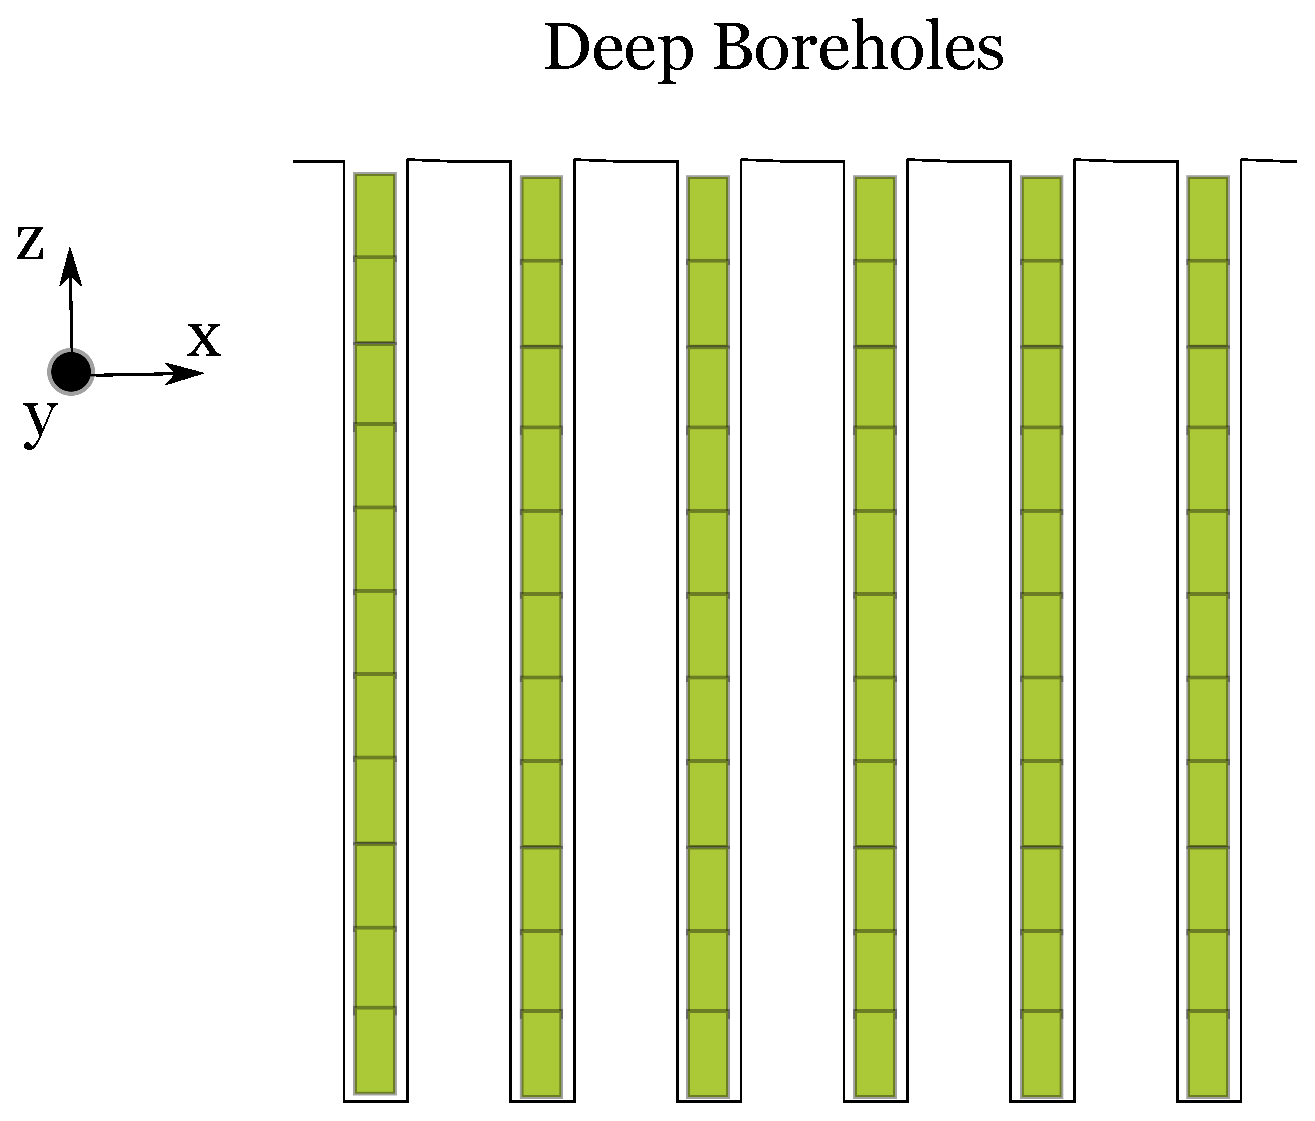
\includegraphics[width=\textwidth]{boreholes.eps}
    \end{figure}
    \begin{figure}[h!]
      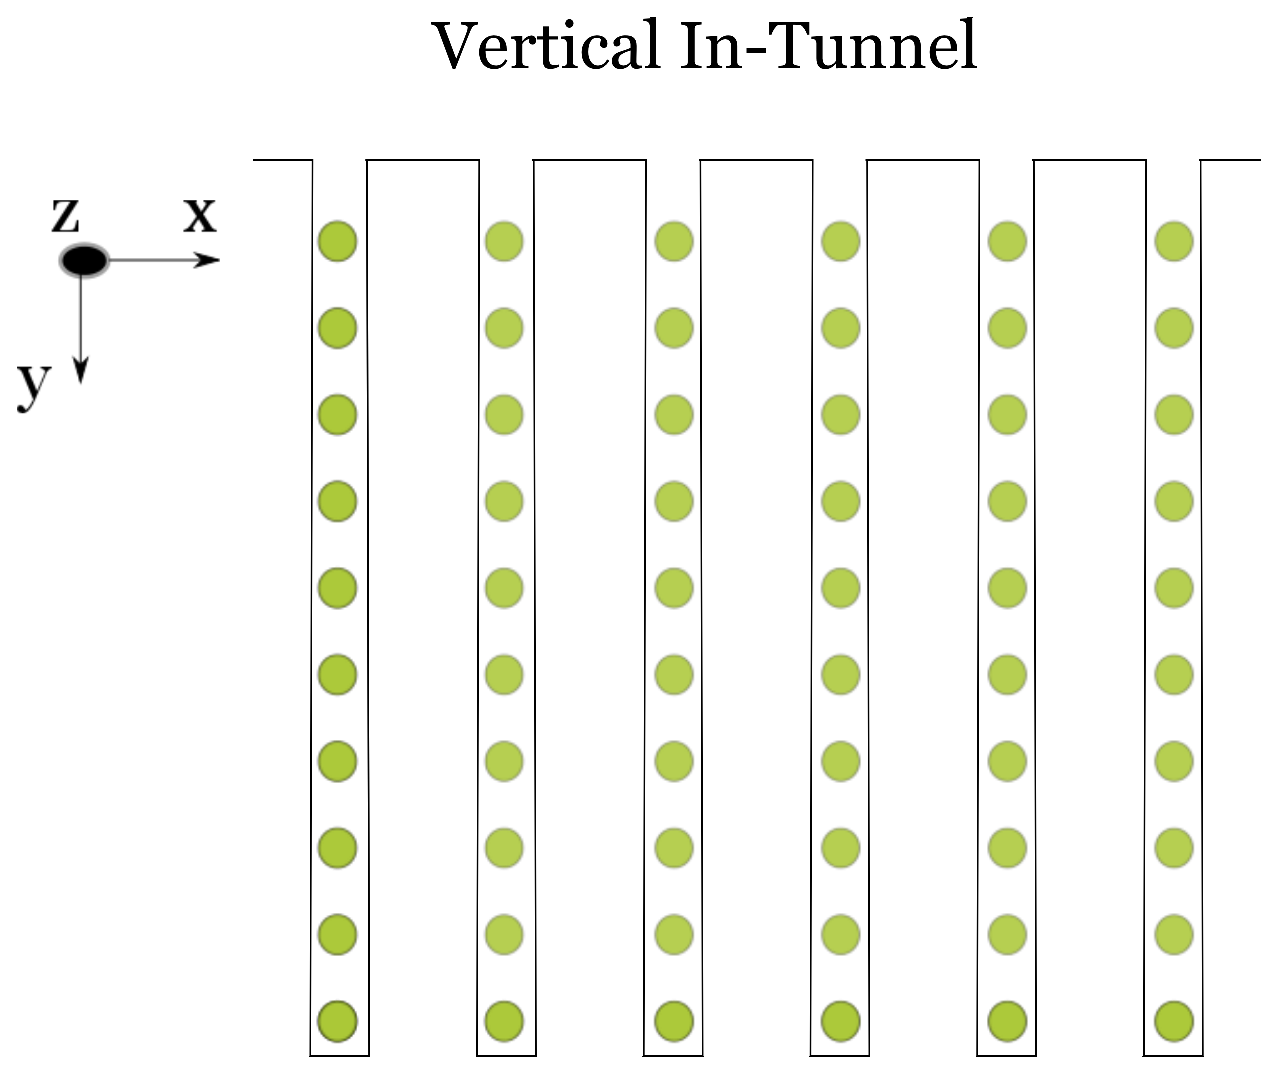
\includegraphics[width=\textwidth]{vertical.eps}
    \end{figure}
  \end{minipage}
  \hspace{0.01cm}
  \begin{minipage}{0.3\textwidth}
    \begin{figure}[h!]
      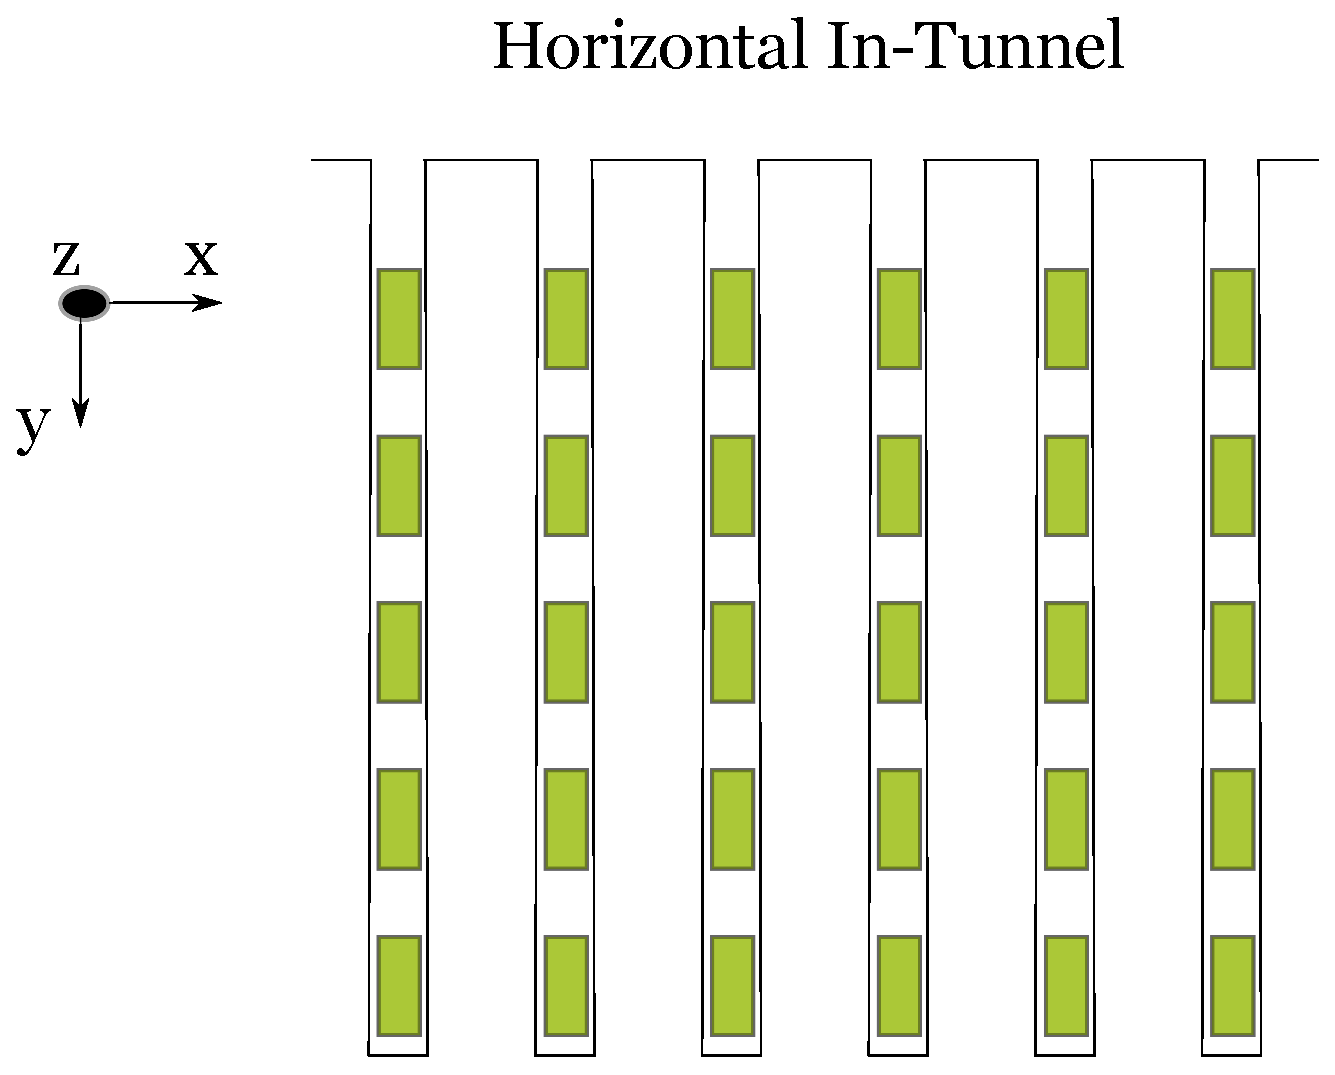
\includegraphics[width=\textwidth]{horizontal.eps}
    \end{figure}
    \begin{figure}[h!]
      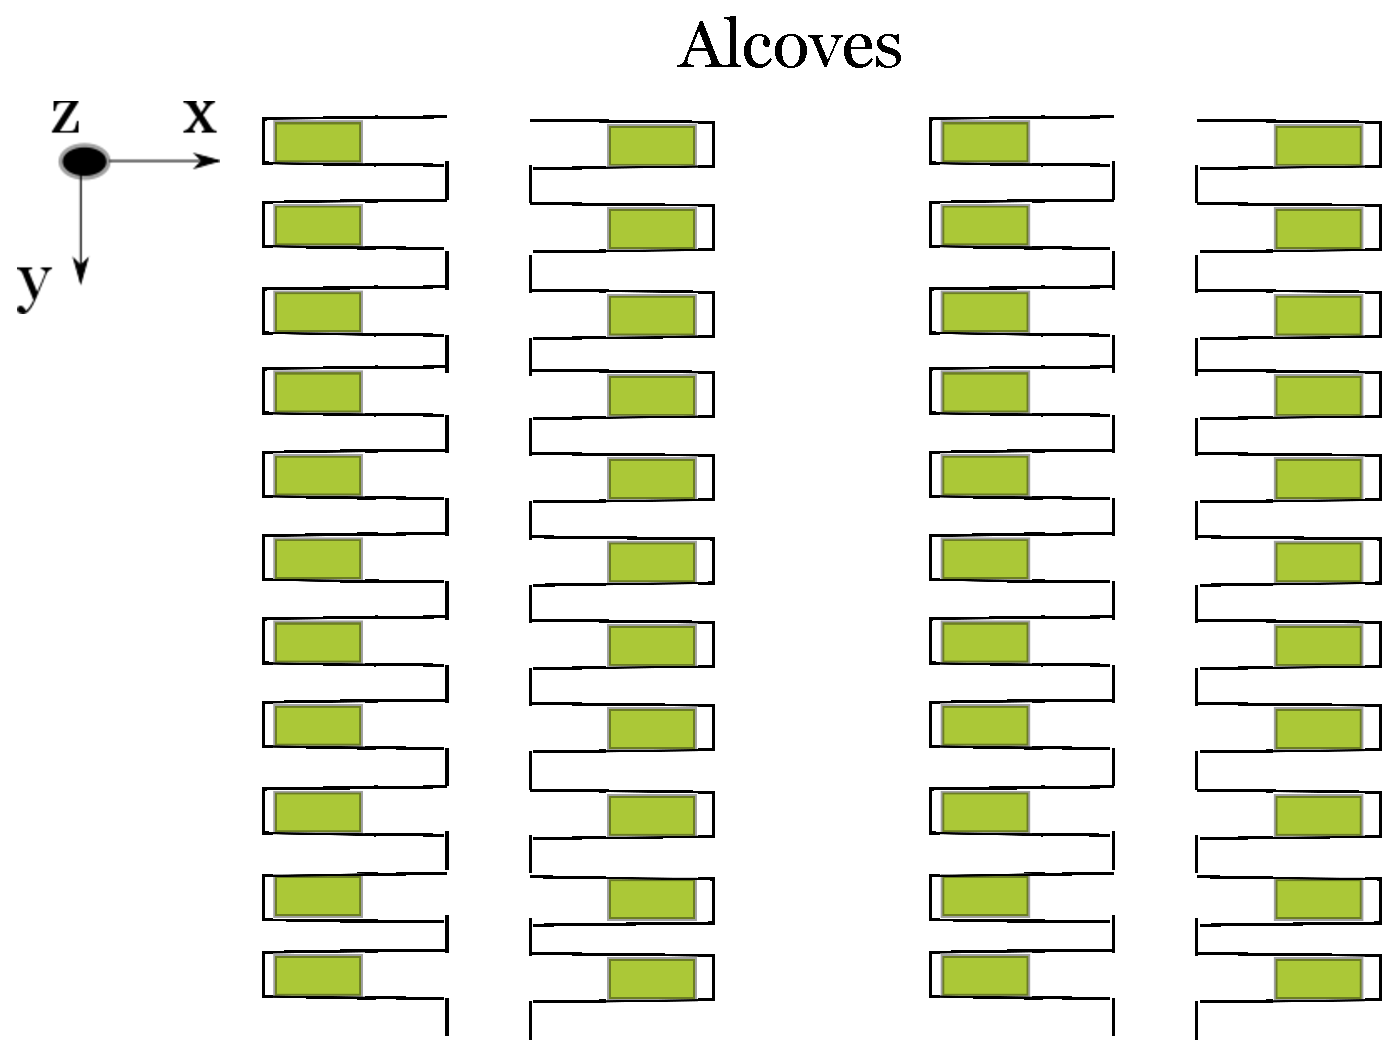
\includegraphics[width=\textwidth]{alcoves.eps}
    \end{figure}
  \end{minipage}
  \hspace{0.01cm}\large{$=$}\hspace{0.01cm}
  \begin{minipage}{0.3\textwidth}
    \begin{figure}[b]
      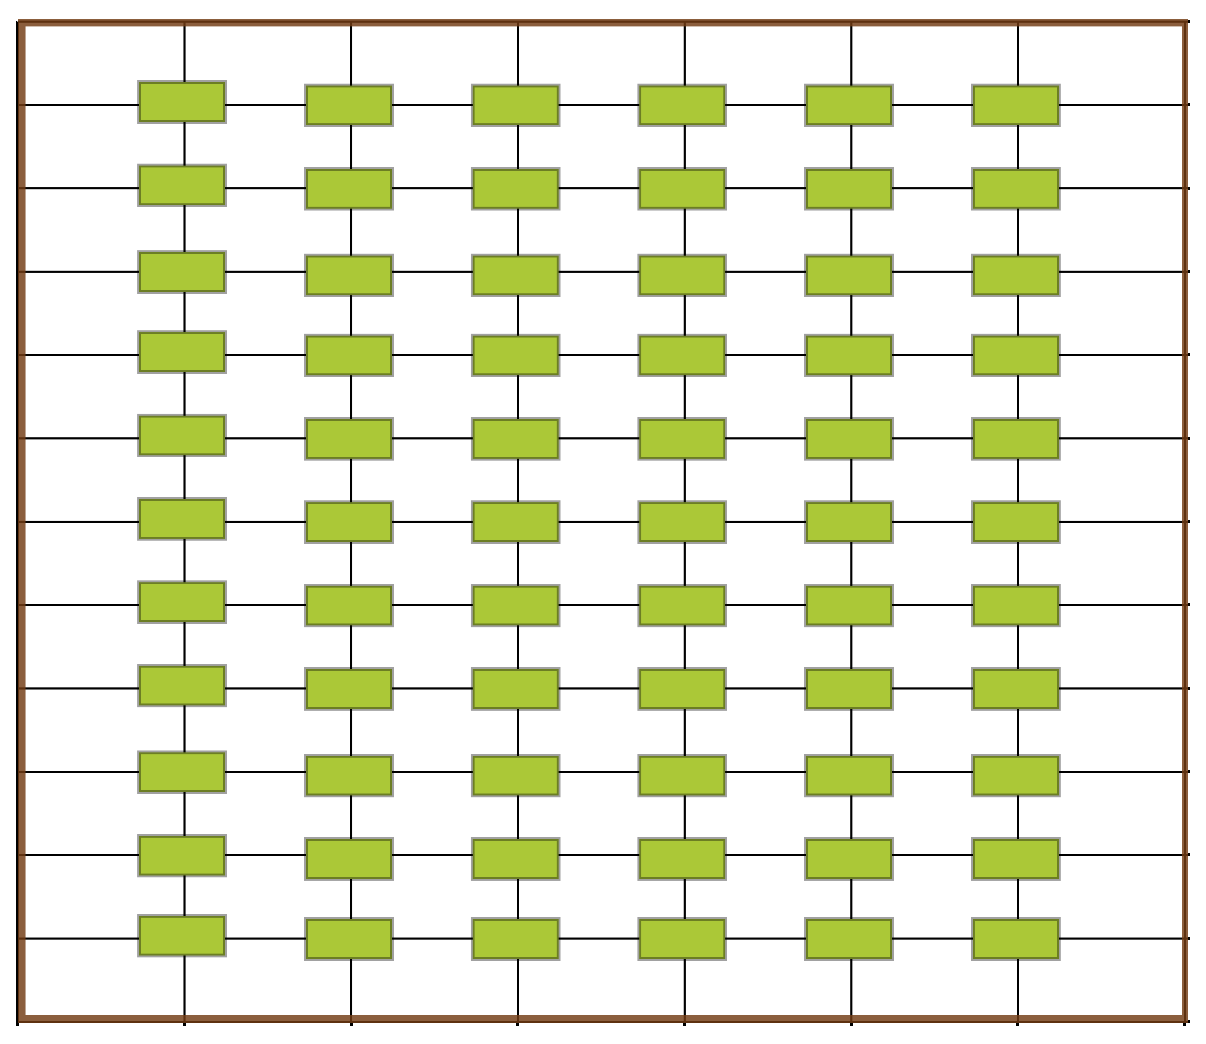
\includegraphics[width=\textwidth]{fullGrid.eps}
    \end{figure}
  \end{minipage}
\end{frame}

\begin{frame}
  \frametitle{LLNL Model : Geometry}
  \begin{figure}[h!]
    \begin{center}
      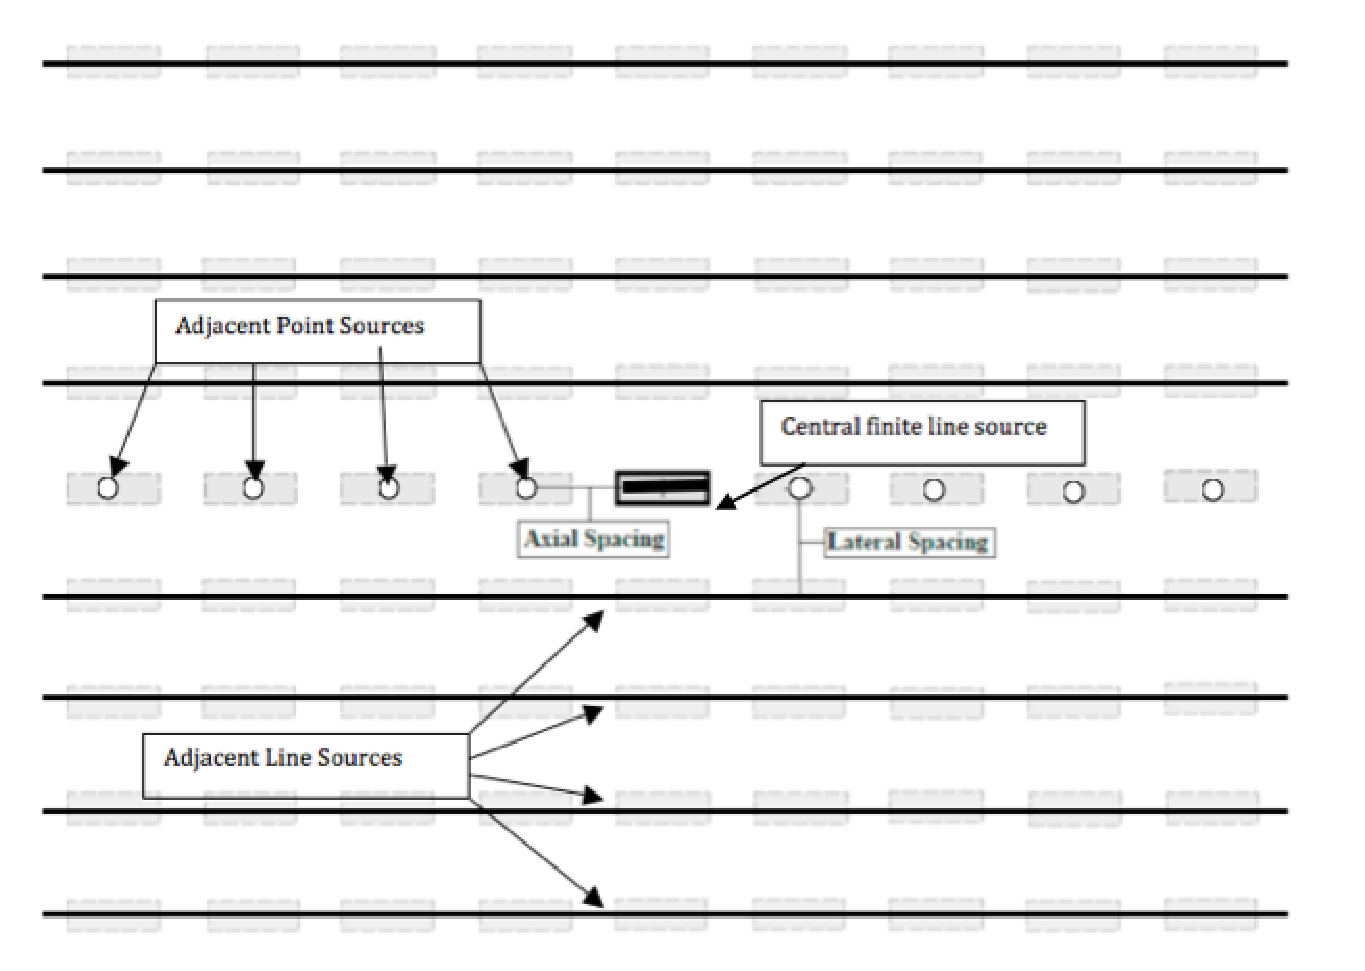
\includegraphics[width=0.7\textwidth]{llnlConcept.eps}
    \end{center}
    \caption{Vertical, horizontal, alcove, and borehole emplacement layouts can 
    be represented by a line of point sources and adjacent line sources 
    \cite{sutton_investigations_2011}.}
    \label{fig:llnl}
  \end{figure}
\end{frame}

\begin{frame}
  \frametitle{LLNL Model : Solution Strategy}
  \footnotesize{
    LLNL's model is a MathCAD solution of the transient homogeneous 
    conduction equation,
    
    \begin{align}
      \nabla^2T  = \frac{1}{\alpha}\frac{\partial T}{\partial t},
      \label{condGl}
    \end{align}
    
    in which superimposed point and line source solutions approximate the repository 
    layout.
    The solution of this equation at the 
    boundary of the EBS and the waste package is then treated as a boundary condition 
    for the heterogeneous steady state equation, 
    
    \begin{align}
      \dot{q} &= U A_{out} \left( T_{in} - T_{out} \right)
      \label{condGeneral}
      \intertext{where}
      U&=\frac{1}{\sum_{i}R_i}
      \intertext{which, for the detailed EBS becomes}
      U&=\frac{1}{R_{WF}+R_{WP}+R_{buffer}+\cdots}
    \end{align}
    
    which calculates a resulting temperature gradient through the geometry at each 
    point in time for each layer surface, assuming an infinite line source 
    \cite{hardin_generic_2011}\cite{sutton_investigations_2011}. 
    }
\end{frame}



